% -*- coding: utf-8; -*-

\chapter{Introduction}
There are several reasons that motivate the adoption of statically typed languages. Maintaining large systems built with dynamic types can become a nightmare due to the lack of type information \cite{takikawa_is_2016}. Typed languages has also generally better performance because compile-time type information helps generating optimized machine code. However, programmers are frequently left empty-handed when inspecting dynamically typed code while having to re-write systems to a statically typed languaged if gradually typed languages are not an option.
\paragraph*{}
Inspired by the challenge of inspecting dynamically typed code, we built a type extractor for the Lua programming language. By inspecting a program's execution during runtime, it can generate enough information to help programmers visualize the types being transfered between functions of their program. The software output can be used as an useful documentation, while also helping programmers migrate code to a statically typed one or even for debugging.
\paragraph*{}
The document is structured as follows. In Chapter ~\ref{cha:Previous Work} we present previous work related to type systems in Lua. In Chapter ~\ref{cha:Project Scope} we describe the software goal. Chapter ~\ref{cha:Project Specification} explain the software modules and how they interact. In Chapter ~\ref{cha:Development} it's shown the software key functions, the modules relationship and basic utilization. In Chapter ~\ref{cha:Results} we present and discuss some results obtained by the type extractor on some Lua benchmarks. Finally on Chapter ~\ref{cha:Final Considerations} we present our conclusion and future work.

% \begin{figure}
% \centering
% 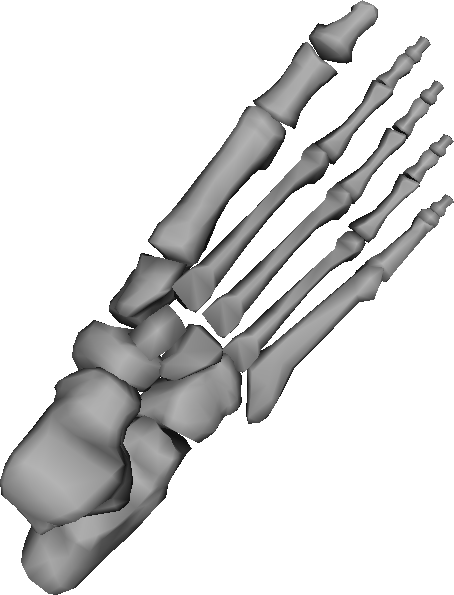
\includegraphics[width=0.45\textwidth]{pictures/image01.png}
% 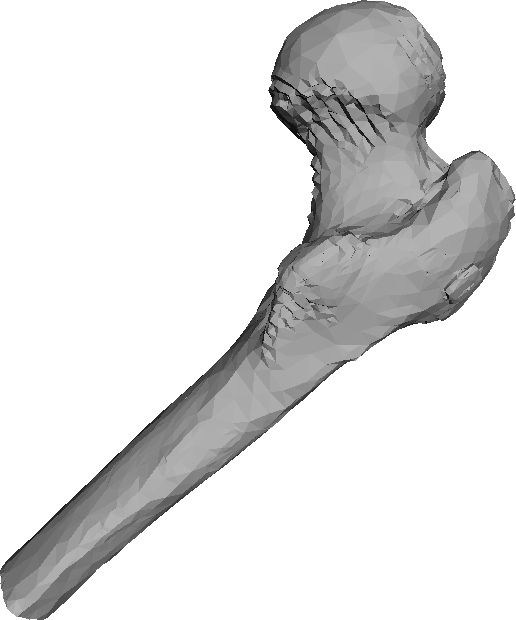
\includegraphics[width=0.45\textwidth]{pictures/image02.png}
% \caption{Meshes generated from medical data. Data obtained from the AIM$@$SHAPE Shape Repository \cite{AIMSHAPE}}
% \label{fig:example}
% \end{figure}

%This document is structured as follows. In Chapter~\ref{cha:Previous Work} we present some previous work relevant to our problem. In Chapter~\ref{cha:Proposal} we explain our proposal. In Chapter~\ref{cha:Results} we show our results. Finally, in Chapter~\ref{cha:Conclusion} we present our conclusion and future work.


